\documentclass{beamer}
\usetheme{Hannover}
\usecolortheme{rose}
\usepackage[utf8]{inputenc} 
\usepackage[english, ngerman]{babel}
\usepackage{tikz,standalone}


\title{Particle Swarm Optimization}
\author[Badertscher, Dengler]{Hannes Badertscher, Gregor Dengler}
\date [MathSem, FS13]{MathSem, \today}


% Aufzählungen immer schrittweise zeigen:
\beamerdefaultoverlayspecification{<+->}
% Gliederung am Anfang jedes unterabschnittes anzeigen:
\AtBeginSubsection[]
{
  \begin{frame}<beamer>
    \frametitle{Gliederung}
    \tableofcontents[currentsection,subsection]
  \end{frame}
}

\begin{document}

	\begin{frame}
		\titlepage
	\end{frame}

	\begin{frame}
		\frametitle{Table of Contents}
		\tableofcontents[currentsection]
	\end{frame}
  
	\section{Einführung}
\begin{frame}{Einführung}
	\begin{itemize}
		\item Schwarm
			\only<1>{
				\begin{figure}[htbp]
					\centering
					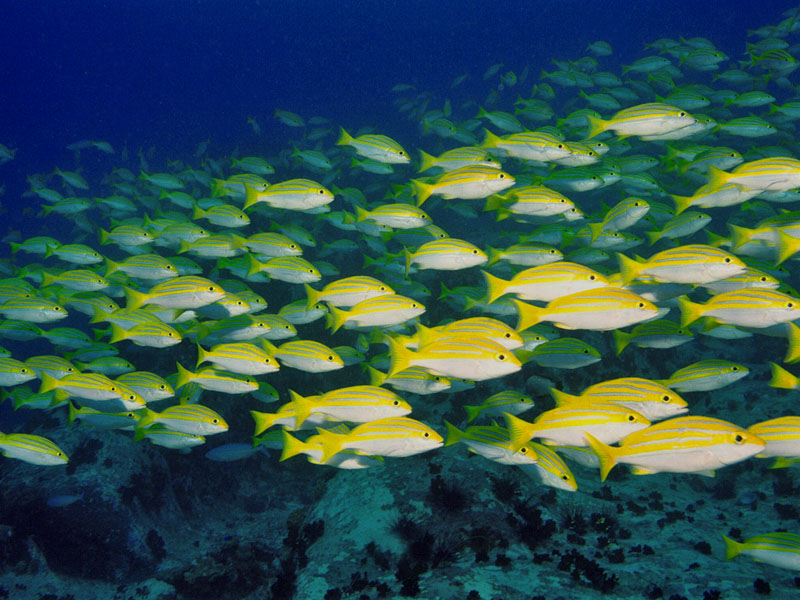
\includegraphics[width=5cm]{Bilder/Schwarm.jpg}
				\end{figure}
			}
		\item Schwarmintelligenz
			\only<2>{
				\begin{figure}[htbp]
					\centering
					
\includegraphics[width=5cm]{Bilder/Schwarmintelligenz.jpg}
				\end{figure}
			}
		\item Emergenz
		\item Schwarmalgorithums
\end{itemize}
\end{frame}
	\begin{frame}
	\frametitle{Partikelschwarm Algorithmus}
	
	\section[Algorithmus]{Partikelschwarm Algorithmus}
	Zustandsdaten jedes Partikels:
	\begin{align*}
		x_i: \: \: & \text{aktuelle Position}\\
		v_i: \: \: & \text{aktuelle Geschwindigkeit}\\
		p_i: \: \: & \text{Persönlich beste Position} \\
		l_i: \: \: & \text{Beste Position des Schwarms}
	\end{align*}
	

	Initialisierung:
	\begin{align*}
		x_i(0) &= U(min,max) \\
		v_i(0) &= U(min - x_i(0), max - x_i(0)) \\
		p_i(0) &= x_i(0)
	\end{align*}
	
\end{frame}

\begin{frame}
	\frametitle{Partikelschwarm Algorithmus}
	Geschwindigkeits- und Positions-Update:
	\begin{align*}
		v_i(t+1) &= w v_i(t) \\
				&+ U(0,c_1) \left(p_i(t)-x_i(t) \right) \\
				&+ U(0,c_2) \left(l_i(t)-x_i(t) \right) \\
		x_{i}(t+1) &= x_i(t) + v_i(t+1)
	\end{align*}

	\begin{align*}
		w &: \text{Intertia Weight} \\
		c_1 &: \text{Cognitive Factor} \\
		c_2 &: \text{Social Factor} \\
		U(a,b) &: \text{Random Number between a,b}
	\end{align*}	
\end{frame}

\begin{frame}
	\frametitle{Partikelschwarm Algorithmus}
	Visualisierung
	\begin{figure}[htbp]
		\documentclass{standalone}

\usepackage{tikz}
\usetikzlibrary{arrows,decorations.pathmorphing,positioning,fit,petri}
\usetikzlibrary{calc,intersections,through,backgrounds,graphs}
\usetikzlibrary{patterns,decorations.pathreplacing}

\begin{document}

\begin{tikzpicture}
	% Styles
	[
	point/.style={circle,draw=blue!50,fill=blue!20,thick, inner sep=0pt,minimum size=4mm},
	vpoint/.style={circle,draw=gray!50,fill=gray!20,thick, inner sep=0pt,minimum size=4mm},
	endpoint/.style={circle,draw=red!50,fill=red!20,thick, inner sep=0pt,minimum size=4mm},
	]
                      
	% Axis
	\draw[->] (0,0) -- (5,0);
  	\draw[->] (0,0) -- (0,5);
	
	% Shaded Parts
	\fill[gray!10!yellow!10] (1,1.5) rectangle (4.3,5.02);
	\fill[gray!10!green!10] (1,1.5) rectangle (4.85,0.4);

	% Nodes
	\node at (1.5,4.5)	(xi1)	[vpoint]	{};
	\node at (3,1.2)	(xi2)	[vpoint]	{};
	\node at (4,4.7)	(pi)	[point] 	{};
	\node at (4.5,0.5)	(li)	[point] 	{};
	\node at (1.7,-1)	(wvi) [point]	{};
	\node at (1,1.5)	(xi)	[point]	{} 
		edge [->,densely dotted]			(xi1)
		edge[densely dotted,gray]		(4.3,5.02)
		edge[->,densely dashdotted]		(xi2)
		edge[densely dashdotted,gray]	(4.85,0.4);
	\node at (4.2,1.7)	(xit)	[endpoint] {};
	\draw[->] (xi) -- (wvi);
	\draw[->,densely dotted] (wvi)  -- (2.2,2);
	\draw[->,densely dashdotted] (2.2,2) -- (xit);
	\draw[->,red!50]	(xi) -- (xit);

	% Text
	\node[blue!50]		at (0.6,1.5)	{$x_i$};
	\node[gray!50]		at (1.1,4.5) 	{$x'_i$};
	\node[gray!50]		at (3.5,1.2) 	{$x''_i$};
	\node[blue!50]		at (4,4.2)		{$p_i$};
	\node[blue!50]		at (4.2,0.2)	{$l_i$};
	\node[red!50]		at (4.2,2.2)	{$x_i(t+1)$};
	\node[blue!50]		at (1.1,-0.5)	{$wv_i$};

\end{tikzpicture}

\end{document}
	\end{figure}
\end{frame}
	\section{Schwarm-Topologien}
\begin{frame}{Schwarm-Topologien}
	\begin{figure}[htbp]
		\centering
		\begin{minipage}{4cm}
			\centering
			\documentclass{standalone}

\usepackage{tikz}
\usetikzlibrary{arrows,decorations.pathmorphing,positioning,fit,petri}
\usetikzlibrary{calc,intersections,through,backgrounds,graphs}
\usetikzlibrary{patterns,decorations.pathreplacing}

\begin{document}

\begin{tikzpicture}
	% Styles
	[
	place/.style={circle,draw=blue!50,fill=blue!20,thick, inner sep=0pt,minimum size=4mm},
	]
                      
	% Nodes
	\node at (0,0.5)	(p1)	[place] {};
	\node at (0,1.5)	(p2)	[place] {};
	\node at (1,0)		(p3)	[place] {};
	\node at (1,2)		(p4)	[place] {};
	\node at (2,0.5)	(p5)	[place] {};
	\node at (2,1.5)	(p6)	[place] {};
	
	% Connections
	\graph[use existing nodes] {
		p1 -- p2; p1 -- p3; p1 -- p4; p1 -- p5; p1 -- p6;
		p2 -- p3; p2 -- p4; p2 -- p5; p2 -- p6;
		p3 -- p4; p3 -- p5; p3 -- p6;
		p4 -- p5; p4 -- p6;
		p5 -- p6;
	};
	

\end{tikzpicture}

\end{document}
			GBest
		\end{minipage}
		\begin{minipage}{4cm}
			\centering
			\documentclass{standalone}

\usepackage{tikz}
\usetikzlibrary{arrows,decorations.pathmorphing,positioning,fit,petri}
\usetikzlibrary{calc,intersections,through,backgrounds,graphs}
\usetikzlibrary{patterns,decorations.pathreplacing}

\begin{document}


\begin{tikzpicture}
	% Styles
	[
	place/.style={circle,draw=blue!50,fill=blue!20,thick, inner sep=0pt,minimum size=4mm},
	]
                      
	% Nodes
	\node at (0,0.5)	(p1)	[place] {};
	\node at (0,1.5)	(p2)	[place] {};
	\node at (1,0)		(p3)	[place] {};
	\node at (1,2)		(p4)	[place] {};
	\node at (2,0.5)	(p5)	[place] {};
	\node at (2,1.5)	(p6)	[place] {};
	
	% Connections
	\graph[use existing nodes] {
		p1 -- p2 -- p4 -- p6 -- p5 -- p3 -- p1;
	};
	

\end{tikzpicture}

\end{document}
			LBest - Ring
		\end{minipage}
		\begin{minipage}{4cm}
			\centering
			\documentclass{standalone}

\usepackage{tikz}
\usetikzlibrary{arrows,decorations.pathmorphing,positioning,fit,petri}
\usetikzlibrary{calc,intersections,through,backgrounds,graphs}
\usetikzlibrary{patterns,decorations.pathreplacing}

\begin{document}

\begin{tikzpicture}
	% Styles
	[
	place/.style={circle,draw=blue!50,fill=blue!20,thick, inner sep=0pt,minimum size=4mm},
	]
                      
	% Nodes
	\node at (0,0.5)	(p1)	[place] {};
	\node at (0,1.5)	(p2)	[place] {};
	\node at (1,0)		(p3)	[place] {};
	\node at (1,2)		(p4)	[place] {};
	\node at (2,0.5)	(p5)	[place] {};
	\node at (2,1.5)	(p6)	[place] {};
	
	% Connections
	\graph[use existing nodes] {
		p4 -- p1;
		p4 -- p2;
		p4 -- p3;
		p4 -- p5;
		p4 -- p6;
	};
	

\end{tikzpicture}

\end{document}
			LBest - Wheel
		\end{minipage}
		\begin{minipage}{4cm}
			\centering
			\documentclass{standalone}

\usepackage{tikz}
\usetikzlibrary{arrows,decorations.pathmorphing,positioning,fit,petri}
\usetikzlibrary{calc,intersections,through,backgrounds,graphs}
\usetikzlibrary{patterns,decorations.pathreplacing}

\begin{document}

\begin{tikzpicture}
	% Styles
	[
	place/.style={circle,draw=blue!50,fill=blue!20,thick, inner sep=0pt,minimum size=4mm},
	]
                      
	% Nodes
	\node at (0,0)	(p1)	[place] {};
	\node at (0,1)	(p2)	[place] {};
	\node at (0,2)	(p3)	[place] {};
	\node at (1,0)	(p4)	[place] {};
	\node at (1,1)	(p5)	[place] {};
	\node at (1,2)	(p6)	[place] {};
	\node at (2,0)	(p7)	[place] {};
	\node at (2,1)	(p8)	[place] {};
	\node at (2,2)	(p9)	[place] {};
	
	% Connections
	\graph[use existing nodes] {
		p1 -- p2 -- p3;
		p4 -- p5 -- p6;
		p7 -- p8 -- p9;
		p1 -- p4 -- p7;
		p2 -- p5 -- p8;
		p3 -- p6 -- p9;
	};

\end{tikzpicture}

\end{document}
			LBest - Von Neumann
		\end{minipage}
	\end{figure}		
\end{frame}

\section[Zielgebiet]{Einschränkung des Zielgebiets}
\begin{frame}{Einschränkung des Zielgebiets}
	\begin{itemize}
		\item Warum eine Einschränkung ?
		\item Wie schränkt man ein Zielgebiet ein ?
		\begin{itemize}
			\item Apprallen lassen
			\item Fitness Wert auf schlechten Wert setzten
			\item Geschwindigkeit an den Grenzen auf Null setzten
		\end{itemize}
	\end{itemize}
\end{frame}

\section[Geschwindigkeit]{Maximale Geschwindigkeit}
\begin{frame}{Maximale Geschwindigkeit}
	\begin{itemize}
		\item Schnell hohe Geschwindigkeiten
		\item Lösungsansatz: Maximale Geschwindigkeit $V_{max,j}$
			\begin{equation*}
				v_{ij}(t+1) = 
				\begin{cases}
					v_{ij}(t+1) & \text{if} |v_{ij}(t+1)| < V_{max,j} \\
					V_{max,j} & \text{if} |v_{ij}(t+1)| \geq V_{max,j}
				\end{cases}
			\end{equation*} 
	\end{itemize}
\end{frame}

\section[Abbruch-kriterien]{Abbruchkriterien}
\begin{frame}{Abbruchkriterien}
	\begin{itemize}
		\item Maximale Anzahl Iterationen
			\only<1>{\\ \ \\ \ \\ 
				\colorbox{YellowGreen}{for(int i = 0, i \textless \ Maximale Anzahl Iterationen, i++)}
			}
		
		\item Schwellwert für Fitnesswert
			\only<2>{\\ \ \\ \ \\ 
				\colorbox{YellowGreen}{if(global best \textgreater \ Schwellwert) \{ ... \} }
			}
		
		\item Schwellwert für Änderung der Funktionswerte
			\only<3>{\\ \ \\ \ \\ 
				\colorbox{YellowGreen}{if(Minimale Geschwindikeit \textless \ Schwellwert)}
			}
		
		\item Schwellwert für Bewegungsbereich
			\only<4>{\\ \ \\ \ \\ \ \\
			}
		
	\end{itemize}
\end{frame}
	\section{Anwendungen}
\begin{frame}{Anwendungen}
	\begin{itemize}
		\item Analyse neuraler Netzwerke
				\only<1>{\\ \ \\ \ \\ 
					\colorbox{YellowGreen}{Diagnose von Parkinson}}
		\item Zucht von Mikroorganismen
				\only<2>{\\ \ \\ \ \\ 
					\colorbox{YellowGreen}{Zusammensetzung der Nährstoffe}}
		\item Objektlageerkennung in Tiefendaten	
	\end{itemize}
\end{frame}

\begin{frame}{Anwendungen}
	\begin{itemize}
		\item Ausgangslage
				\only<1>{
					\begin{figure}
						\begin{minipage}{4.5cm}
							\centering
							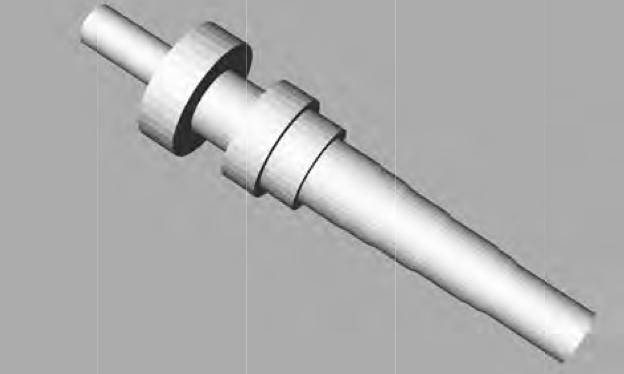
\includegraphics[width=4cm]{Bilder/welle-cad} \\
							CAD-Modell einer Getriebewelle
						\end{minipage}
						\begin{minipage}{4.5cm}
							\centering
							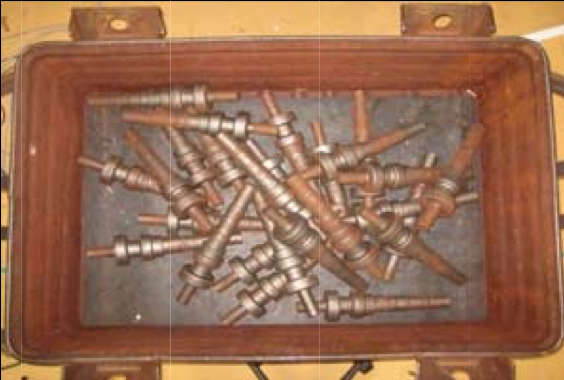
\includegraphics[width=4cm]{Bilder/welle-kiste} \\
							Beispiel einer Kiste mit Getriebewellen zur Ultraschallprüfung
						\end{minipage}
					\end{figure}
				}
		\item Objektorientierung $R_i$	
			\only<2>{
				\begin{figure}
					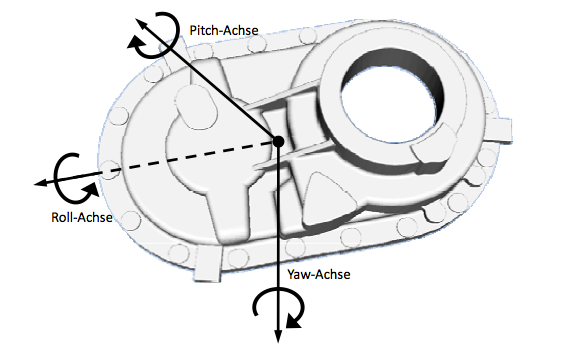
\includegraphics[width=5cm]{Bilder/yaw-pitch-roll}
				\end{figure}
			}
		\item Objektposition $P_i$
			\only<3>{\\ \ \\ 
				\colorbox{YellowGreen}{Referenzpunkt: höchster Punkt}}
		\item Objektmerkmalsdaten $C_i$
			\only<4>{\\ \ \\ 
				\colorbox{YellowGreen}{Segmentierung der Tiefendaten}}
		\item Fitnessfunktion: $f(p_i) = f(R_i,P_i,C_i)$
			\only<5>{\\ \ \\
				\colorbox{YellowGreen}{Vergleich mit Histogrammen aus Wissensbasis}}
		\item Schwarm
			\only<6>{\\ \ \\
				\colorbox{YellowGreen}{100 Partikel, lbest mit 30 Nachbarn, 100 Iterationen}}
		\item Resultat
			\only<7>{\\ \ \\
				\colorbox{YellowGreen}{Dauer: 4s, Erkennungsrate $>92\%$}}
	\end{itemize}
\end{frame}
	\section[Demonstration]{Demonstration C++ Code}

\begin{frame}{C++ Code}
	\begin{itemize}
		\item Position-Klasse
			\only<1>{\\ \ \\ \ \\ 
				\colorbox{YellowGreen}{Mehrdimensionaler Datentyp}}
		\item Particle-Klasse
			\only<2>{\\ \ \\ \ \\ 
				\colorbox{YellowGreen}{Modellierung eines einzelnen Partikels}}
		\item Swarm-Klasse
			\only<3>{\\ \ \\ \ \\ 
				\colorbox{YellowGreen}{Modellierung des Schwarmverhaltens}}
	\end{itemize}
\end{frame}

\begin{frame}{Visualisierung mit Matlab}
	\foreach \index in {1, ..., 20} 
	{
	  \only<\index>{\includegraphics[width=\textwidth]{Bilder/frames/Frame\index.png}}
	}
\end{frame}

\end{document}